% !TeX root = ../main.tex

\chapter{实验过程与分析}

\section{实验过程}

\subsection{实验环境}
本实验使用Pycharm完成。

操作系统:Win10。

硬件:处理器为i7-7700(主频4.2GHz),显卡为NVIDIA TITAN X(Pascal架构显存12G),内存容量为32G(速度2400MHz)。

软件:代码运行在Pycharm上,使用Pytorch框架。

\subsection{数据集}
本实验数据集为在1-3米分辨率下的遥感图像,总共4615张图片。每张图片如图\ref{DataSetExample}所示:

\begin{figure}
	\center
	{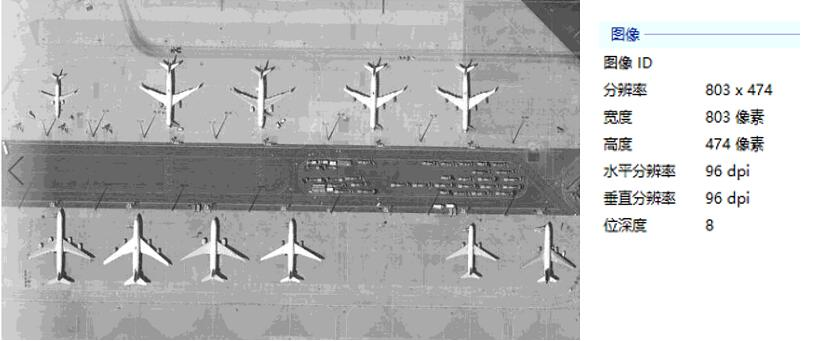
\includegraphics[width=16cm,height=7cm]{DataSetExample.jpg}}
	\caption{遥感图像数据集样例}
	\label{DataSetExample}
\end{figure}

每张图片的含有关于飞机、油库、船具体坐标的标注(作为$Ground Truth$),如图\ref{Annoation}所示:

\begin{figure}
	\center
	{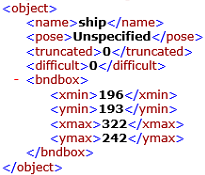
\includegraphics[width=4cm,height=4cm]{Annoation.png}}
	\caption{人工标注示例}
	\label{Annoation}
\end{figure}

\subsection{评价指标}

本实验的评价指标包括每个类的召回率$Reacall$、平均准确率$AP$以及三个类的$MeanAP$。

\subsubsection{混淆矩阵}

我们通常使用混淆矩阵来评估一个二分类问题。混淆矩阵会把样本实例分为正类($positive$)与负类($negative$)。在训练测试开始前我们已经有了$Ground Truth$的信息,然后根据使用训练完成的模型来对测试集进行处理,输出每张图片上的检测结果。对于图像目标检测问题来说,它对正、负类的评价标准是这个图片上该位置处物体的类别信息是否与$Ground Truth$相同,并且在类别检测正确后判断IOU是否达到阈值,如果大于等于阈值就认为该检测结果是正类。因此,对测试结果评估这个二分类问题而言,检测结果会出现以下四种情况:

真正类($True \ Positive,TP$),测试输出的结果为正类的正样本。

假正类($False \ Positive,FP$),测试输出的结果为正类的负样本。

假负类($False \ Negative,FN$),测试输出的结果为负类的正样本。

真负类($True \ Negative,TN$),测试输出的结果为负类的负样本。

如图\ref{HXMatrix}所示。

\begin{figure}
	\center
	{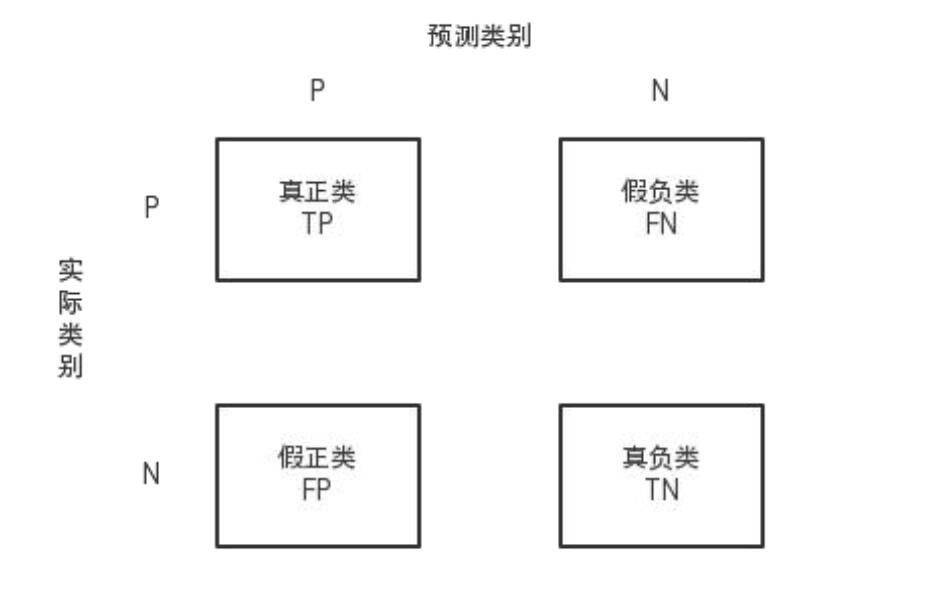
\includegraphics[width=9.46cm,height=5.96cm]{HXMatrix.jpg}}
	\caption{混淆矩阵}
	\label{HXMatrix}
\end{figure}

\subsubsection{准确率与召回率}

准确率($Precision$)是所有测试输出为正的样本(正真类与假正类)在总样本数中的占比,用$P$表示,其计算方式如下:

\begin{equation}
	P=\frac{TP+TN}{TP+FP+FN+TN}
\end{equation}


召回率($Recall$)是真正类在所有正类(正真类与假负类)中的占比,在公式中用$R$表示,计算方式如下:

\begin{equation}
R=\frac{TP}{TP+FN}
\end{equation}

准确率与召回率的定义可以由图\ref{PreRec}直观感受。

\begin{figure}
	\center
	{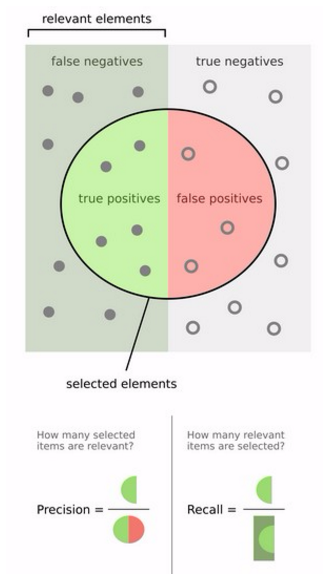
\includegraphics[width=7cm,height=12cm]{PreRec.png}}
	\caption{准确率、召回率的定义}
	\label{PreRec}
\end{figure}

\subsubsection{$AP$与$MAP$}

上面讲述了$Precision$和$Recall$的含义,而我们需要一个同时考虑准确率与召回率的指标。

$AP$($Average\ Precision$):平均准确率,在不同$recall$下的最高$precision$的准确率(一般会对各类别分别计算各自的$AP$)。

$mAP$($mean\ AP$):平均准确率的均值,各类别的$AP$的均值。

试想,如果在一个$Bounding Box$里,检测器识别出来某类$T$的$score$最高,可是结果也只有$0.1$,那么它很可能还是负样本。 所以我们需要一个阈值,如果识别出了T类而且分数大于这个阈值才说明它是正样本,否则它是负样本。阈值影响$Precision$和$Recall$的方式如下所述。在$T$类的例子中,如果阈值太高,$Prediction$非常严格,所以我们认为是T类的基本都是$T$类,$Precision$就高了;但也因为筛选太严格,我们也放过了一些$score$比较低的$T$类,所以$Recall$就低了;如果阈值太低,什么都会被当成$T$类,$Precision$就会很低,而$Recall$会很高。这样我们就明确了阈值确实对$T$类的$Precision$和$Recall$产生影响和变化的趋势,也就说明,$Precision$不是一个绝对的东西,而是相对阈值而改变的东西,$Recall$同理。那么单个用$Precision$来作为标准判断,就不合适。需要综合考虑$Precision$与$Recall$之间的关系,用一组固定值表述不够全面, 因为我们根据不同的阈值, 可以取到不同(也可能相同)的$Precision-Recall$值。 这样想的话对于每个阈值,我们都有相应的($Precision$,$Recall$)对,也就有了$Precision$和$Recall$之间的曲线关系。这样一条“$P-R$曲线”,它衡量着两个有价值的判断标准,即$Precision$和$Recall$的关系,将这两个指标一起动态考虑,就有了$T$这个类的$Average Precision$,即曲线下的面积,他可以充分的表示在这个模型中,$Precision$和$Recall$的总体优劣。最后,我们计算每个类的$Average Precision$,就得到了$Mean\ Average\ Precision$。

故$AP$衡量的是学出来的模型在具体某个类别上检测结果的好坏,而$mAP$衡量的是学习的模型在所有类别上的结果。

\section{实验分析}

\subsection{训练细节}

本实验检测飞机、油库、船三类;总类数还要加上背景,故$num\_class=4$

$labelmap = ('airplane', 'ship', 'storage\_tank')$

$VOC\_CLASSES = ('\_\_background\_\_', 'airplane', 'ship', 'storage\_tank')$

训练集使用总图片数的$80\%$,3694张;测试集使用总图片数的$20\%$,921张。

\subsection{检测结果}

本实验总共训练110个$Epoch$,每10个$Epoch$进行一次$Loss$、$MAP$、每类的$AP$输出(由于到第100个$Epoch$后出现$Loss$升高、$MAP$降低的过拟合现象,故展现前100个$Epoch$的结果),如表\ref{EpoMAP}、表\ref{EpoLoss}、图\ref{DisAP}所示。

\begin{table}
	\caption{训练Epoch与MAP的关系}
	\begin{tabular}{ccccccccccc}
		\hline
		Epoch & 10 & 20 & 30 & 40 & 50 & 60 & 70 & 80 & 90 & 100 \\
		\hline
		MAP & 0.3759 & 0.7331 & 0.8085 & 0.8288 & 0.8127 & 0.8371 & 0.8325 & 0.8216 & 0.8446 & 0.8507 \\
		\hline
	\end{tabular}
	\label{EpoMAP}
\end{table}

\begin{table}
	\caption{训练Epoch与Loss的关系}
	\begin{tabular}{ccccccccccc}
		Epoch & 10 & 20 & 30 & 40 & 50 & 60 & 70 & 80 & 90 & 100 \\
		\hline
		Loss & 0.4290 & 0.3726 & 0.3439 & 0.3116 & 0.2996 & 0.2859 & 0.2713 & 0.2632 & 0.2602 & 0.2586 \\
		\hline
	\end{tabular}
	\label{EpoLoss}
\end{table}

\begin{figure}[htbp]
	\subfigure[storage\_tank类的平均准确率]{
		\begin{minipage}{4.6cm}
			\centering
			{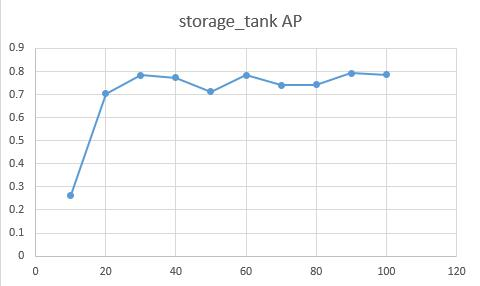
\includegraphics[width=5.5cm,height=3.2cm]{storageAP.jpg}}
		\end{minipage}
	\label{DisAP1}
	}
	\subfigure[ship类的平均准确率]{
		\begin{minipage}{4.6cm}
			\centering
			{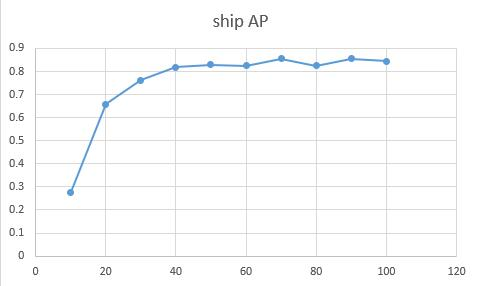
\includegraphics[width=5.5cm,height=3.2cm]{shipAP.jpg}}
		\end{minipage}
	\label{DisAP2}
	}
	\subfigure[airplane类的平均准确率]{
		\begin{minipage}{4.6cm}
			\centering
			{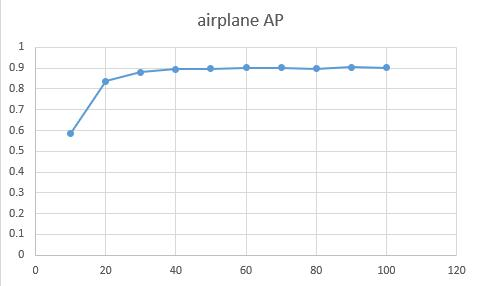
\includegraphics[width=5.5cm,height=3.2cm]{airplaneAP.jpg}}
		\end{minipage}
	\label{DisAP3}
	}
	\caption{各类AP值与Epoch的关系}
	\label{DisAP}
\end{figure}

训练完100个$Epoch$后各类的$Recall$、$AP$值如表\ref{RecAP}所示,每个类的$Recall$都很高,说明绝大部分的目标都被检测出来了。同时各类的$AP$也很高,说明在综合准确率召回率的情况下该网络检测的效果非常好,验证了ASSD算法的有效性。

\begin{table}
	\caption{各类Recall与AP值}
	\centering
	\begin{tabular}{cccc}
		\hline
		information & airplane & ship & stroage\_tank\\
		\hline
		Recall & 0.9640 & 0.9387 & 0.8741\\
		AP & 0.9029 & 0.8453 & 0.7857\\
		\hline
	\end{tabular}
	\label{RecAP}
\end{table}

从训练过程中的输出可以看出$Loss$在不断降低$MAP$在不断升高,故选择第100个$Epoch$的结果进行后面的可视化处理。

\subsection{可视化结果}

训练过程中记录下该模型中的各项权重,执行完100个$Epoch$后调用可视化程序对验证集中的图片进行查看,其效果如图\ref{DisPic}所示:
\begin{figure}[htbp]
	\centering
	\subfigure[storage\_tank]{
		\begin{minipage}{4.6cm}
			\centering
			{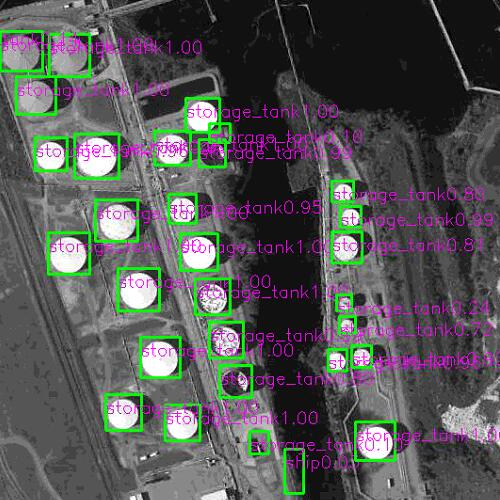
\includegraphics[width=4.8cm,height=4.8cm]{vis1.jpg}}
		\end{minipage}
	}
    \subfigure[ship]{
    	\begin{minipage}{4.6cm}
    		\centering
    		{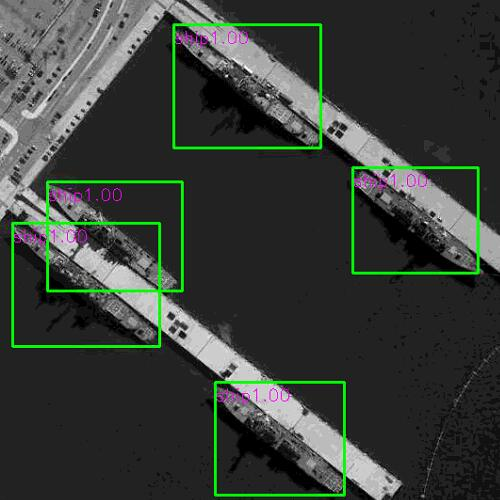
\includegraphics[width=4.8cm,height=4.8cm]{vis2.jpg}}
    	\end{minipage}
    }
	\subfigure[airplane]{
		\begin{minipage}{4.6cm}
			\centering
			{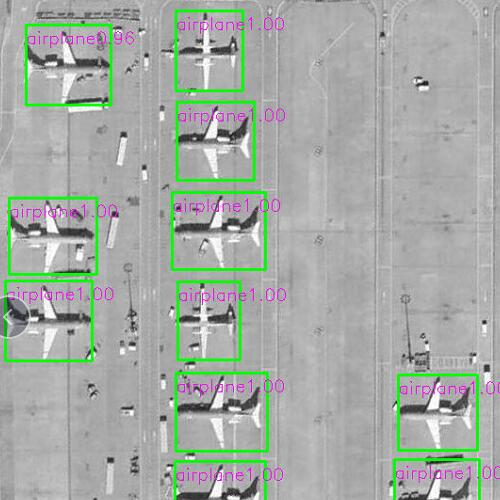
\includegraphics[width=4.8cm,height=4.8cm]{vis3.jpg}}
		\end{minipage}
	}
	\caption{各类可视化检测结果}
	\label{DisPic}
\end{figure}

其中各类的识别与其轮廓的标注都很符合$Ground$ $Truth$,可见检测效果还是很不错的。即ASSD通过使用语义融合机制与注意力机制在遥感图像数据集上实现了较好的表现效果。

